% sage_latex_guidelines.tex V1.01, 11 June 2015


% choose journal options here
\documentclass[Royal,sageh,times]{sagej}

\usepackage{moreverb,url}

\usepackage[colorlinks,bookmarksopen,bookmarksnumbered,citecolor=red,urlcolor=red]{hyperref}

\newcommand\BibTeX{{\rmfamily B\kern-.05em \textsc{i\kern-.025em b}\kern-.08em
T\kern-.1667em\lower.7ex\hbox{E}\kern-.125emX}}

\def\volumeyear{2016}



%%%%%%%%%%%%%%%%%%%%%%%
%% User-defined commands
%%%%%%%%%%%%%%%%%%%%%%%

% Operators
\DeclareMathOperator{\Cov}{Cov}
\DeclareMathOperator{\Var}{Var}
\DeclareMathOperator{\E}{\mathbb{E}}
\DeclareMathOperator{\Proba}{\mathbb{P}}

\newcommand{\Covb}[2]{\ensuremath{\Cov\!\left[#1,#2\right]}}
\newcommand{\Eb}[1]{\ensuremath{\E\!\left[#1\right]}}
\newcommand{\Pb}[1]{\ensuremath{\Proba\!\left[#1\right]}}
\newcommand{\Varb}[1]{\ensuremath{\Var\!\left[#1\right]}}

% norm
\newcommand{\norm}[1]{\| #1 \|}




\setcounter{secnumdepth}{3}


%%%%%%%%%%%%%%%%%%%%%%%
\begin{document}

\runninghead{Raimbault J.}

\title{Indirect Evidence of Network Effects in a System of Cities}

\author{Juste Raimbault\affilnum{1}\affilnum{2}}

\affiliation{\affilnum{1}UMR CNRS 8504 G{\'e}ographie-cit{\'e}s, Paris, France\\
\affilnum{2}UMR-T IFSTTAR 9403 LVMT, Champs-sur-Marne, France}

\corrauth{Juste Raimbault, UMR CNRS 8504 G{\'e}ographie-cit{\'e}s
13 rue du Four,
75006 Paris, France.}

\email{juste.raimbault@polytechnique.edu}

\begin{abstract}
This paper is the application of a theoretical paper developing a theory of co-evolutive networked territorial systems. We apply simple models of urban growth for systems of cities, which include in particular the role of physical networks.
\end{abstract}

\keywords{Urban Systems, Urban Growth, Spatial Interactions}

\maketitle


%%%%%%%%%%%%%%%%%%%




%%%%%%%%%%%%%%%%%%%%%%%%
\section{Introduction}

%%%%%%%%%%%%%%%%%%%%%%%%
\subsection{Modeling Urban Growth}

Understanding processes driving urban growth is more crucial than ever, as urban population recently crossed the symbolic proportion of half world population~\cite{}.% TODO cite ? 
 Future of world economies and sustainability of future societies seem to be deeply interlinked with the dynamics of urban systems.%cite
 A better knowledge of how cities differentiate, interact and grow is thus a relevant topic both theoretically and for application. Many disciplines have studied models of urban growth with different objectives and taking different aspects into account. Economics still have a difficulty to consider spatial interactions in their models~\cite{krugman1998space}, whereas geography fails to embrace a certain level of complexity. The example of this two disciplines shows how it is difficult to make bridges, as it needed exceptional minds to translate from one to the other (as P. Hall did for Von Thunen work~\cite{taylor2016polymath}) % note : also quote here economic geo/geo economic ?

% broad review from different disciplines point of view
% NOTE : justify scale here (eg not urban sprawl models)


%%%%%%%%%%%%%%%%%%%%%%%%
\subsection{Urban Growth and Spatial Interaction}

% more refined literature on models of urban growth including space


\cite{bretagnolle2000long} already proposed a spatial extension of the Gibrat model. Later, \cite{favaro2011gibrat} developed a more refined extension with economic cycles and innovation waves, yielding a system dynamics version of the core of Simpop models.

% marius as an extension of Gibrat ? in the deterministic case.


%%%%%%%%%%%%%%%%%%%%%%%%
\subsection{Urban Growth and Networks}

% idem with networks / transportation networks





% what we propose to do here

We work on simple territorial systems that are country-wide city systems, and more particularly French cities, on a time scale corresponding to that spatial scale, i.e. two last centuries. Taking into account physical networks can improve the understanding of city growth within that system in two ways : a qualitative one, for which the extended model would exhibit qualitative features corresponding to stylized facts empirically observed but that more basic models do not manage to reproduce, and a quantitative way, in the sense that model extension improves explained variance further than the mechanic improvement due to the introduction of supplementary degrees of freedom. If at least one of these is unveiled in our particular case, the evidence will support the theory at these scale and in this context.



The rest of this paper is organized as follows : our model is introduced and formally described in next section ; we then describe results obtained through exploration and calibration of our model on data for french cities, in particular the unveiling of network effects significantly influencing growth processes. We finally discuss interpretations of these results and implications for planning.





%%%%%%%%%%%%%%%%%%%%%%%%%
\section{Model Description}




\subsection{From Gibrat to Marius : the dilemma of formulation}

% stochastic vs deterministic formulation ? precise possible formulations and what choice means.

%  - Gabaix \cite{gabaix1999zipf} details stationary distribution of Gibrat model - link with Zipf law. why we do not accept this "explanation" : NOT stationary. depends on time scales to reach stationarity ?
%  - bayesian iterative formulation ? (mcmc)
%  - how does formulation influence ? equivalence in certain cases between stoch-cov and interdependent expectancies ?



%%%%%%%%%%%%%%%%%%%%%%
\subsection{Model description}

We choose to work on a deterministic extension of the Gibrat model, what is equivalent to consider only expectancies in time as detailed before. Let $\vec{P}(t)=(P_i(t))_i$ be the population of cities in time. Under Gibrat independence assumptions, we have $\Covb{P_i(t)}{P_j(t)}=0$. If $\vec{P}(t+1)=\mathbf{R}\cdot \vec{P}(t)$ where $\mathbf{R}$ is also independent, then $\Eb{\vec{P}(t+1)}=\mathbf{R}\cdot\Eb{\vec{P}}(t)$. With $\vec{\mu}(t)=\Eb{\vec{P}(t)}$, we generalize this approach by taking $\vec{\mu}(t+1)=f(\vec{\mu}(t))$. In our case, we take

\[f(\vec{\mu}) = r_0\cdot \mathbf{Id}\cdot \vec{\mu} + \mathbf{G}\cdot \mathbf{1} + \mathbf{N}\cdot \]

with 
\begin{itemize}
\item $G_{ij} = w_G\cdot \frac{V_{ij}}{<V_{ij}>}$ and $V_{ij} = \left(\frac{\mu_i\mu_j}{\sum{\mu_k}^2}\right)^{\gamma_G} \exp{(-d_{ij}/d_G)}$
\item $N_{i} = w_N \cdot \sum_{kl} \left(\frac{\mu_k\mu_l}{\sum\mu}\right)^{\gamma_N}\exp{(-d_{kl,i})/d_N}$ where $d_{kl,i}$ is distance to shortest path between $k,l$ computed with slope impedance ($Z=\left(1+\alpha/\alpha_0\right)^{n_0}$ with $\alpha_0\simeq 3$)
\end{itemize}

The first component is the pure Gibrat model, that we obtain by setting the weights $w_G = w_N = 0$. The second component captures interdependencies between 






%%%%%%%%%%%%%%%%%%%%%%%%%
\section{Results}

\subsection{Data}


\paragraph{Population data}



%%%%%%%%%%%%%%%%%%%%%%%%%
\begin{figure}
\centering
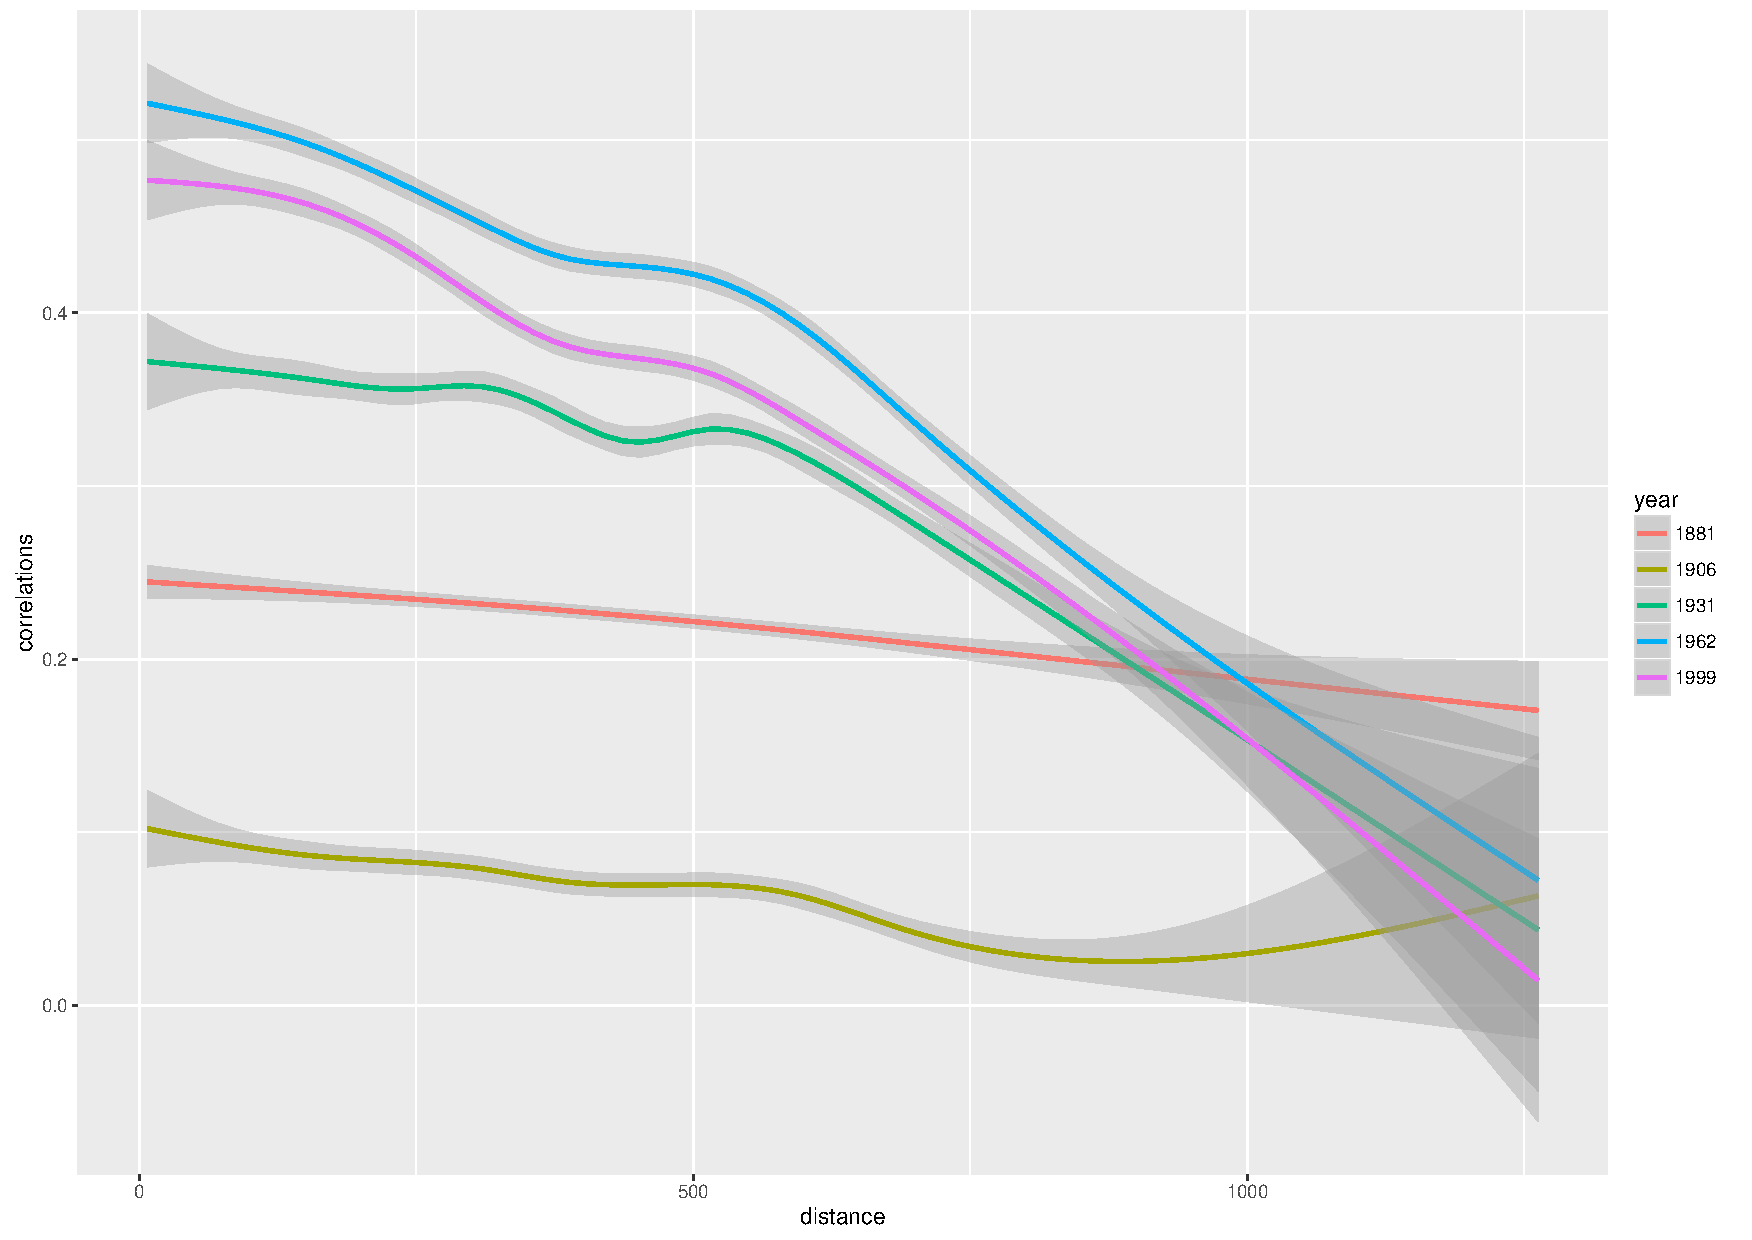
\includegraphics[width=0.8\textwidth]{figures/empirical_tsCorrelations}
\caption{Time-series correlations as a function of distance. Solid line correspond to smoothed correlations, computed between each normalized population time-series, on successive periods.}
\end{figure}
%%%%%%%%%%%%%%%%%%%%%%%%%


\paragraph{Physical flows}

As stated above, this modeling exercise focuses on exploring the role of physical flows, whatever the effective shape of the network. We do not need for this reason network data which is furthermore not easily available at different time periods, and physical flows are assumed to take the geographical shortest path that include terrain slope (to avoid geographical absurdities such as cities with a difficult access having an overestimated growth rate). Using the 1km resolution Digital Elevation Model openly available from IGN~\cite{}%cite bdalti
, we construct an impedance field of the form
\[
Z = \left(1 + \frac{\alpha}{\alpha_0}\right)^{n_0}
\]

We took fixed parameter values $\alpha_0 = 3$ (corresponding to approximatively a 5\% slope) and $n_0 = 3$

% TODO : supplementary material showing paths for different param values ?


%%%%%%%%%%%%%%%%%%%%%%%%%%%
\subsection{Implementation}

Data preprocessing, result processing and models profiling are implemented in R. For performances reasons and an easier integration into the OpenMole software for model exploration~\cite{reuillon2013openmole}, a \texttt{scala} version was also developed. The typical question of trade-off between implementation performance and interoperability appeared quickly as an issue, as a blind exploration and calibration can difficultly provide useful thematic conclusions for that kind of model. Finding an improvement in model fit among one parameter dimension is significant if the geographical situation is visualized and the improvement is confirmed as reasonable and not an absurdity.


%%%%%%%%%%%%%%%%%%%
\begin{figure}
\centering
% figures : netlogo interface / typical output ?
\caption{Example of output of the model. The graphical interface allows to explore interactively on which cities changes operate after a parameter change, what is necessary to interpret raw calibration results.}
\end{figure}
%%%%%%%%%%%%%%%%%%%




%%%%%%%%%%%%%%%%%%%%%%%%%%%
\subsection{Model Exploration}

% qualitative behavior : hierarchy inversions/ trajectories of normalized populations (cf papier Denise Anne etc)
% need of synthetic data ?



%%%%%%%%%%%%%%%%%%%%%%%%%%%
\subsection{Model Calibration}

% here put empirical AIC ?




\section{Discussion}

% how this example illustrates well the theory



We propose to support our hypothesis that \textit{physical transportation networks are necessary to explain the morphogenesis of territorial systems} (aka \textit{Network Necessity}) by showing on a relatively simple case that the integration of physical networks into some models effectively increase their explanative power (being careful on the precise definition of model improvement to avoid overfitting).


%%

% reflexions on iterative calibration, here ?



\begin{acks}
The author would like to thank
\end{acks}





%%%%%%%%%%%%%
%% Biblio
%%%%%%%%%%%%%
\bibliographystyle{SageH}
\bibliography{biblio}






\end{document}
























%%%%%%%%%%%%%%%%%%%%
%% Templates
%%%%%%%%%%%%%%%%%%%%




%
%\subsection{Remarks}
%\begin{enumerate}
%\item[(i)] In \verb"\runninghead" use `\textit{et~al.}' if there
%are three or more authors.
%
%\item[(ii)] For multiple author papers please note the use of \verb"\affilnum" to
%link names and affiliations. The corresponding author details need to be included using the
%\verb+\corrauth+ and \verb+\email+ commands.
%
%\item[(iii)] For submitting a double-spaced manuscript, add
%\verb"doublespace" as an option to the documentclass line.
%
%\item[(iv)] The abstract should be capable of standing by itself,
%in the absence of the body of the article and of the bibliography.
%Therefore, it must not contain any reference citations.
%
%\item[(v)] Keywords are separated by commas.
%
%\item[(vi)] If you are submitting to a \textit{SAGE} journal that requires numbered sections (for example, IJRR), please add the command
%  \verb+\setcounter{secnumdepth}{3}+ just above the \verb+\begin{document}+ line.
%
%\end{enumerate}
%
%




%
%
%\section{The article header information}
%The heading for any file using \textsf{\journalclass} is shown in
%Figure~\ref{F1}. You must select options for the trim/text area and
%the reference style of the journal you are submitting to.
%The choice of \verb+options+ are listed in Table~\ref{T1}.
%
%\begin{table}[h]
%\small\sf\centering
%\caption{The choice of options.\label{T1}}
%\begin{tabular}{lll}
%\toprule
%Option&Trim&Columns\\
%\midrule
%\texttt{shortAfour}& 210 $\times$ 280 mm& Double column\\
%\texttt{Afour} &210 $\times$ 297 mm& Double column\\
%\texttt{MCfour} &189 $\times$ 246 mm& Double column\\
%\texttt{PCfour} &170 $\times$ 242 mm& Double column\\
%\texttt{Royal} &156 $\times$ 234 mm& Single column\\
%\texttt{Crown} &7.25 $\times$ 9.5 in&Single column\\
%\bottomrule
%\end{tabular}\\[10pt]
%\begin{tabular}{ll}
%\toprule
%Option&Reference style\\
%\midrule
%\texttt{sageh}&SAGE Harvard style (author-year)\\
%\texttt{sagev}&SAGE Vancouver style (superscript numbers)\\
%\texttt{sageapa}&APA style (author-year)\\
%\bottomrule
%\end{tabular}
%\end{table}
%
%For example, if your journal is short A4 sized, uses Times fonts and has Harvard style references then you would need\\
%{\small\verb+\documentclass[ShortAfour,times,sageh]{sagej}+}
%
%Most \textit{SAGE} journals are published using Times fonts but if for any reason you have a problem using Times you can
%easily resort to Computer Modern fonts by removing the
%\verb"times" option.





%\begin{figure*}
%\setlength{\fboxsep}{0pt}%
%\setlength{\fboxrule}{0pt}%
%\begin{center}
%\begin{boxedverbatim}
%\documentclass[<options>]{sagej}
%
%\begin{document}
%
%\runninghead{<Author surnames>}
%
%\title{<Initial capital only>}
%
%\author{<An Author\affilnum{1},
%Someone Else\affilnum{2} and
%Perhaps Another\affilnum{1}>}
%
%\affiliation{<\affilnum{1}First and third authors' affiliation\\
%\affilnum{2}Second author affiliation>}
%
%\corrauth{<Corresponding author's name and full postal address>}
%
%\email{<Corresponding author's email address>}
%
%\begin{abstract}
%<Text>
%\end{abstract}
%
%\keywords{<List keywords>}
%
%\maketitle
%
%\section{Introduction}
%.
%.
%.
%\end{boxedverbatim}
%\end{center}
%\caption{Example header text.\label{F1}}
%\end{figure*}



%
%
%
%
%
%%%%%%%%%%%%%%%%%%%%%%%%
%\section{The body of the article}
%
%\subsection{Mathematics} \textsf{\journalclass} makes the full
%functionality of \AmS\/\TeX\ available. We encourage the use of
%the \verb"align", \verb"gather" and \verb"multline" environments
%for displayed mathematics. \textsf{amsthm} is used for setting
%theorem-like and proof environments. The usual \verb"\newtheorem"
%command needs to be used to set up the environments for your
%particular document.
%
%\subsection{Figures and tables} \textsf{\journalclass} includes the
%\textsf{graphicx} package for handling figures.
%
%Figures are called in as follows:
%\begin{verbatim}
%\begin{figure}
%\centering
%\includegraphics{<figure name>}
%\caption{<Figure caption>}
%\end{figure}
%\end{verbatim}
%
%For further details on how to size figures, etc., with the
%\textsf{graphicx} package see, for example, \cite{R1}
%or \cite{R3}.
%
%The standard coding for a table is shown in Figure~\ref{F2}.
%
%\begin{figure}
%\setlength{\fboxsep}{0pt}%
%\setlength{\fboxrule}{0pt}%
%\begin{center}
%\begin{boxedverbatim}
%\begin{table}
%\small\sf\centering
%\caption{<Table caption.>}
%\begin{tabular}{<table alignment>}
%\toprule
%<column headings>\\
%\midrule
%<table entries
%(separated by & as usual)>\\
%<table entries>\\
%.
%.
%.\\
%\bottomrule
%\end{tabular}
%\end{table}
%\end{boxedverbatim}
%\end{center}
%\caption{Example table layout.\label{F2}}
%\end{figure}
%
%\subsection{Cross-referencing}
%The use of the \LaTeX\ cross-reference system
%for figures, tables, equations, etc., is encouraged
%(using \verb"\ref{<name>}" and \verb"\label{<name>}").
%
%\subsection{End of paper special sections}
%Depending on the requirements of the journal that you are submitting to,
%there are macros defined to typeset various special sections. \pagebreak
%
%The commands available are:
%\begin{verbatim}
%\begin{acks}
%To typeset an
%  "Acknowledgements" section.
%\end{acks}
%\end{verbatim}
%\begin{verbatim}
%\begin{biog}
%To typeset an
%  "Author biography" section.
%\end{biog}
%\end{verbatim}
%\begin{verbatim}
%\begin{biogs}
%To typeset an
%  "Author Biographies" section.
%\end{biogs}
%\end{verbatim}
%\begin{verbatim}
%\begin{dci}
%To typeset a "Declaration of
%  conflicting interests" section.
%\end{dci}
%\end{verbatim}
%\begin{verbatim}
%\begin{funding}
%To typeset a "Funding" section.
%\end{funding}
%\end{verbatim}
%\begin{verbatim}
%\begin{sm}
%To typeset a
%  "Supplemental material" section.
%\end{sm}
%\end{verbatim}
%
%\subsection{Endnotes}
%Most \textit{SAGE} journals use endnotes rather than footnotes, so any notes should be coded as \verb+\endnote{<Text>}+.
%Place the command \verb+\theendnotes+ just above the Reference section to typeset the endnotes.
%
%To avoid any confusion for papers that use Vancouver style references,  footnotes/endnotes should be edited into the text.
%


%
%\subsection{References}
%Please note that the files \textsf{SageH.bst} and \textsf{SageV.bst} are included with the class file
%for those authors using \BibTeX. For APA style references please use \textsf{mslapa.bst} which should be part of most modern \TeX\ distributions.
%
%See the above instructions regarding choosing the correct reference option.
%
%%\section{Support for \textsf{\journalclass}}
%%We offer on-line support to participating authors. Please contact
%%us via e-mail at \dots
%%
%%We would welcome any feedback, positive or otherwise, on your
%%experiences of using \textsf{\journalclass}.
%




%
%\section{Copyright statement}
%Please  be  aware that the use of  this \LaTeXe\ class file is
%governed by the following conditions.
%
%\subsection{Copyright}
%Copyright \copyright\ \volumeyear\ SAGE Publications Ltd,
%1 Oliver's Yard, 55 City Road, London, EC1Y~1SP, UK. All
%rights reserved.
%
%\subsection{Rules of use}
%This class file is made available for use by authors who wish to
%prepare an article for publication in a \textit{SAGE Publications} journal.
%The user may not exploit any
%part of the class file commercially.
%
%This class file is provided on an \textit{as is}  basis, without
%warranties of any kind, either express or implied, including but
%not limited to warranties of title, or implied  warranties of
%merchantablility or fitness for a particular purpose. There will
%be no duty on the author[s] of the software or SAGE Publications Ltd
%to correct any errors or defects in the software. Any
%statutory  rights you may have remain unaffected by your
%acceptance of these rules of use.
%
%



%
%
%\begin{thebibliography}{99}
%\bibitem[Kopka and Daly(2003)]{R1}
%Kopka~H and Daly~PW (2003) \textit{A Guide to \LaTeX}, 4th~edn.
%Addison-Wesley.
%
%\bibitem[Lamport(1994)]{R2}
%Lamport~L (1994) \textit{\LaTeX: a Document Preparation System},
%2nd~edn. Addison-Wesley.
%
%\bibitem[Mittelbach and Goossens(2004)]{R3}
%Mittelbach~F and Goossens~M (2004) \textit{The \LaTeX\ Companion},
%2nd~edn. Addison-Wesley.
%
%\end{thebibliography}
%
%





